\documentclass{article}
\usepackage[spanish]{babel}
\usepackage[utf8]{inputenc}
\usepackage[T1]{fontenc}
%\usepackage[spanish]{babel}
\usepackage{graphicx}
\begin{document}
\section{Nodo de alarma}
Los componentes son: 
\begin{itemize}
	\item ESP-01. Este es uno de los módulos más simples que incorpora un ESP8266. Además, trae un par de LEDs, una memoria flash externa de 1MB y una antena WIFI.
	\item Pila CR123A (3V, 1480 mAh). El voltaje de esta pila permite conectarla directamente a la alimentación del microcontrolador, sin usar un regulador de voltaje que implicaria un mayor consumo. 
	\item Buzzer activo. Dispone de un oscilador interno. Al aplicar una tensión constante emite un sonido a una frecuencia fija.  
\end{itemize}
El buzzer y la pila se han soldado a una placa de pruebas (ver figura X) además de una hilera de pines hembra para poder extraer el ESP-01 cuando se quiera programar.

\begin{figure}
\center
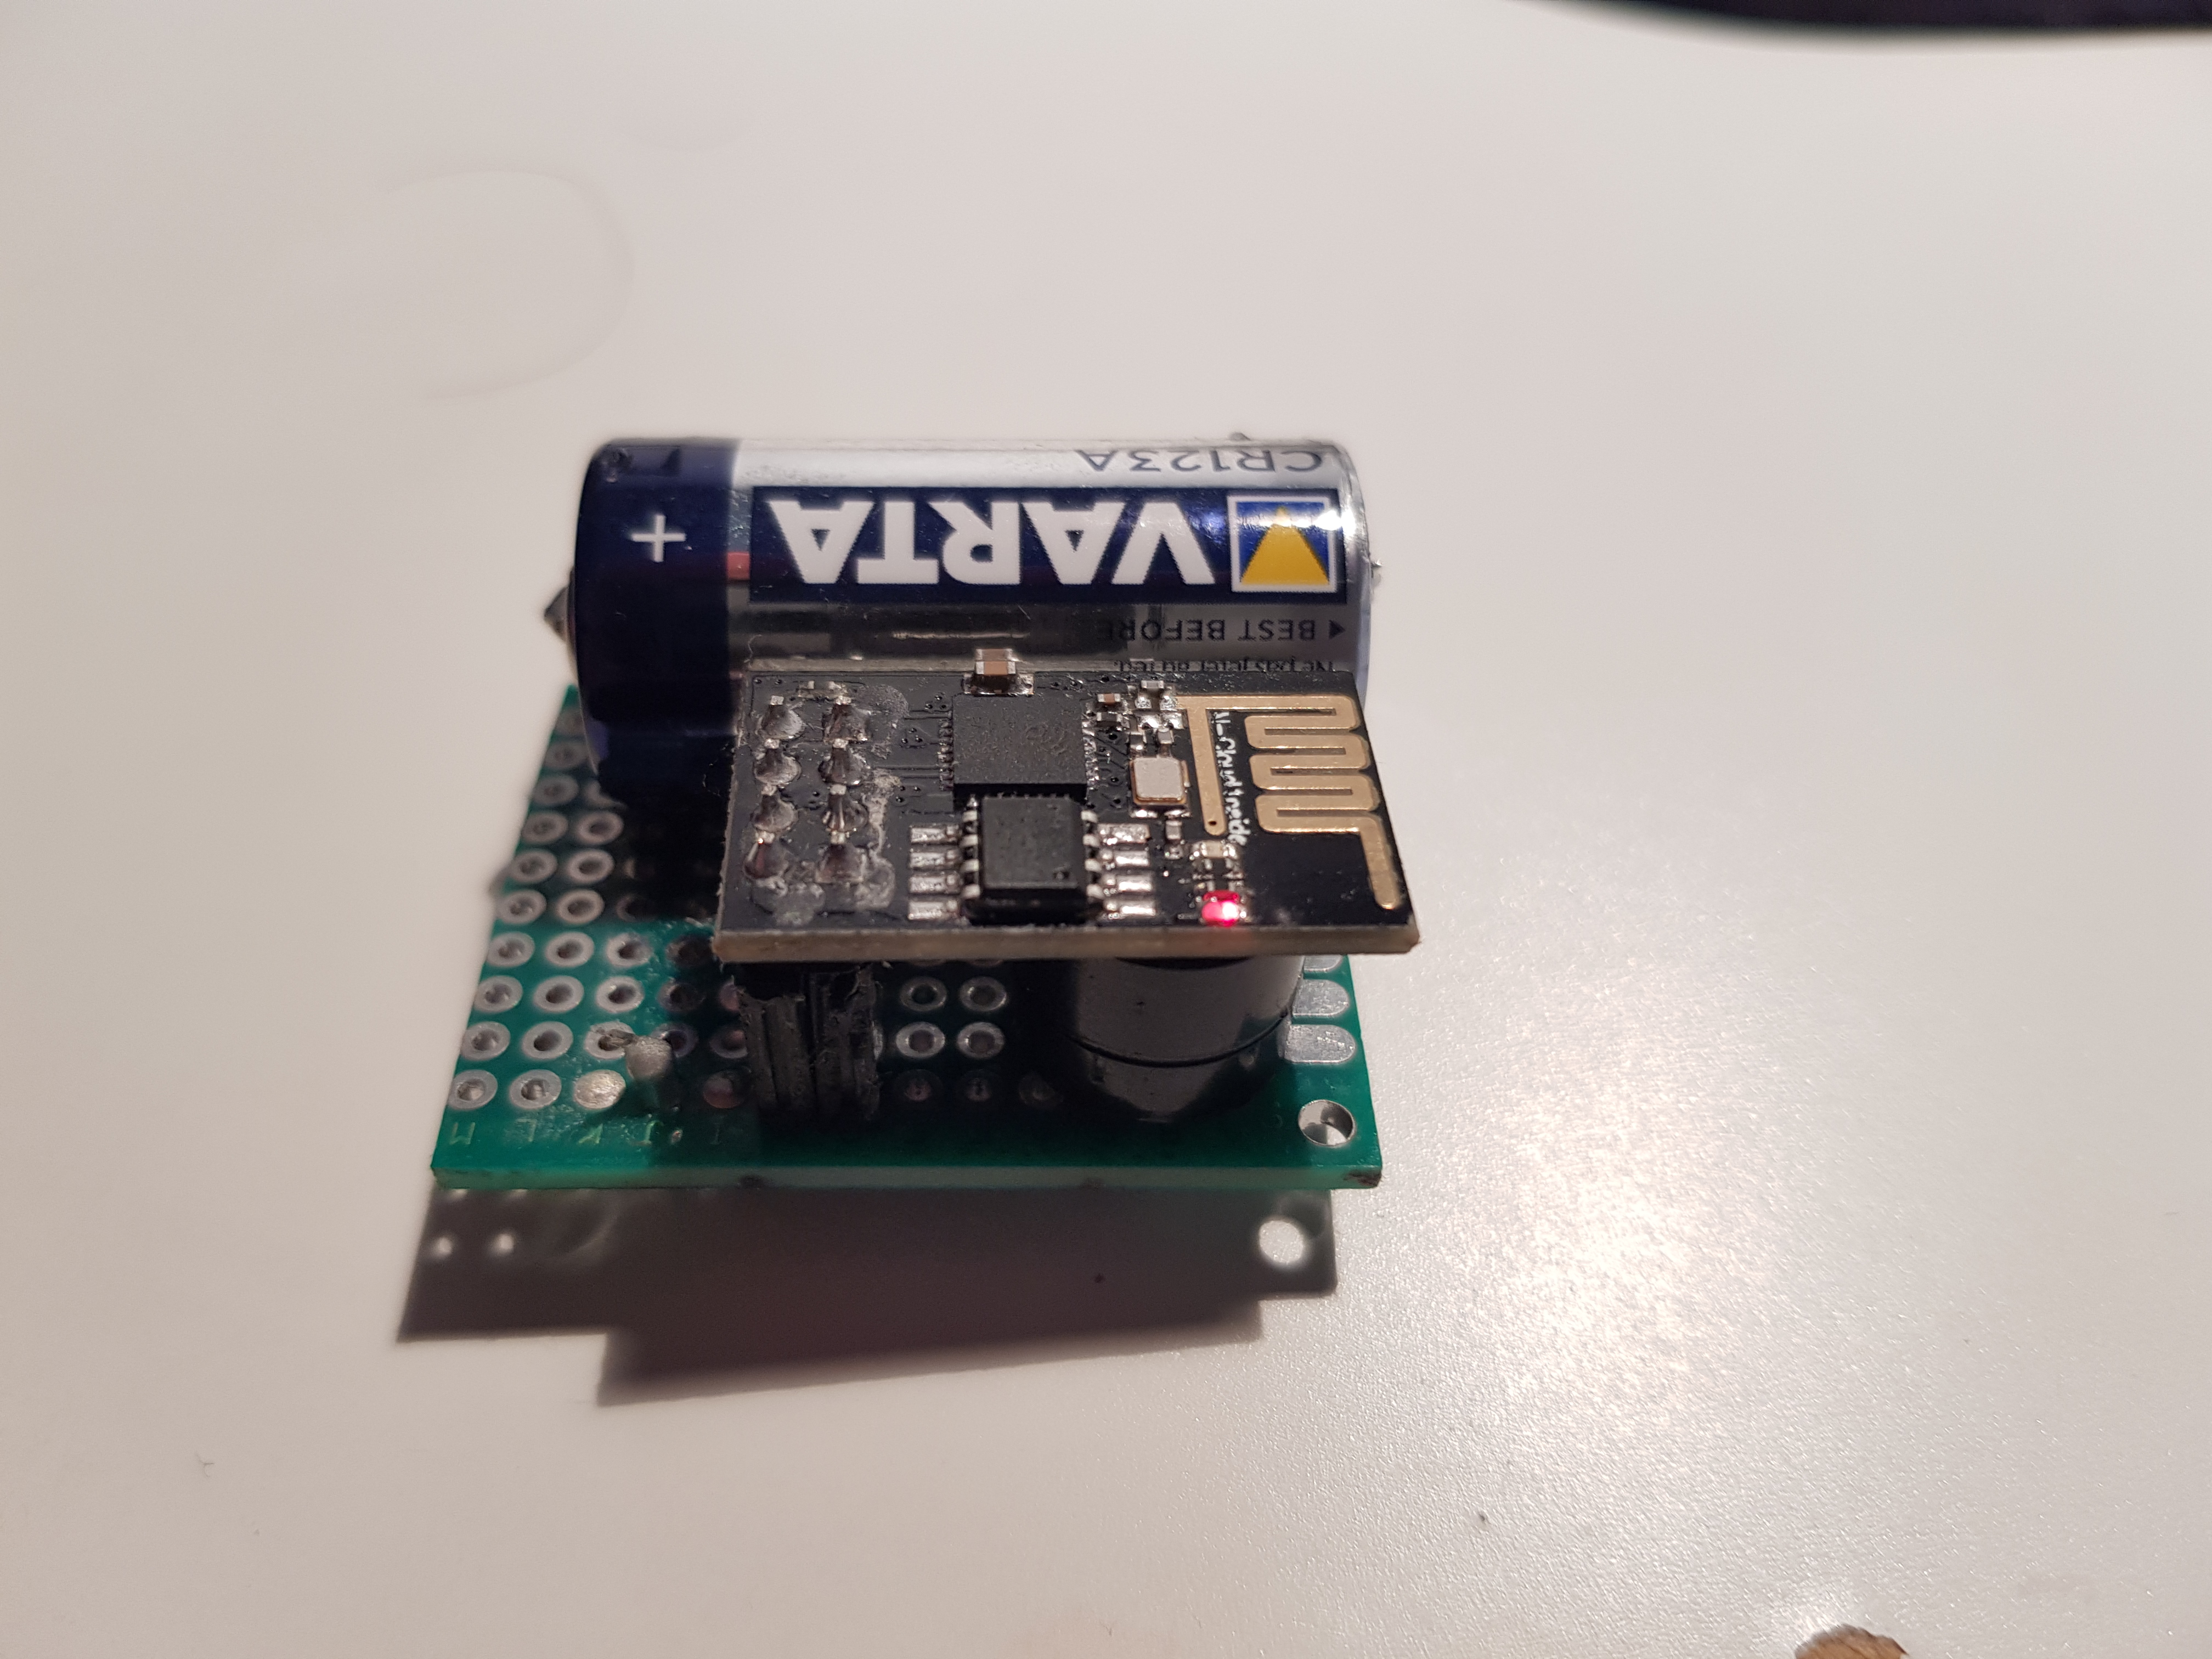
\includegraphics[width=0.5\textwidth]{imagenes/alarma.jpg}
\label{fig:alarma}
\caption{Nodo alarma}
\end{figure}

\begin{figure}
\center
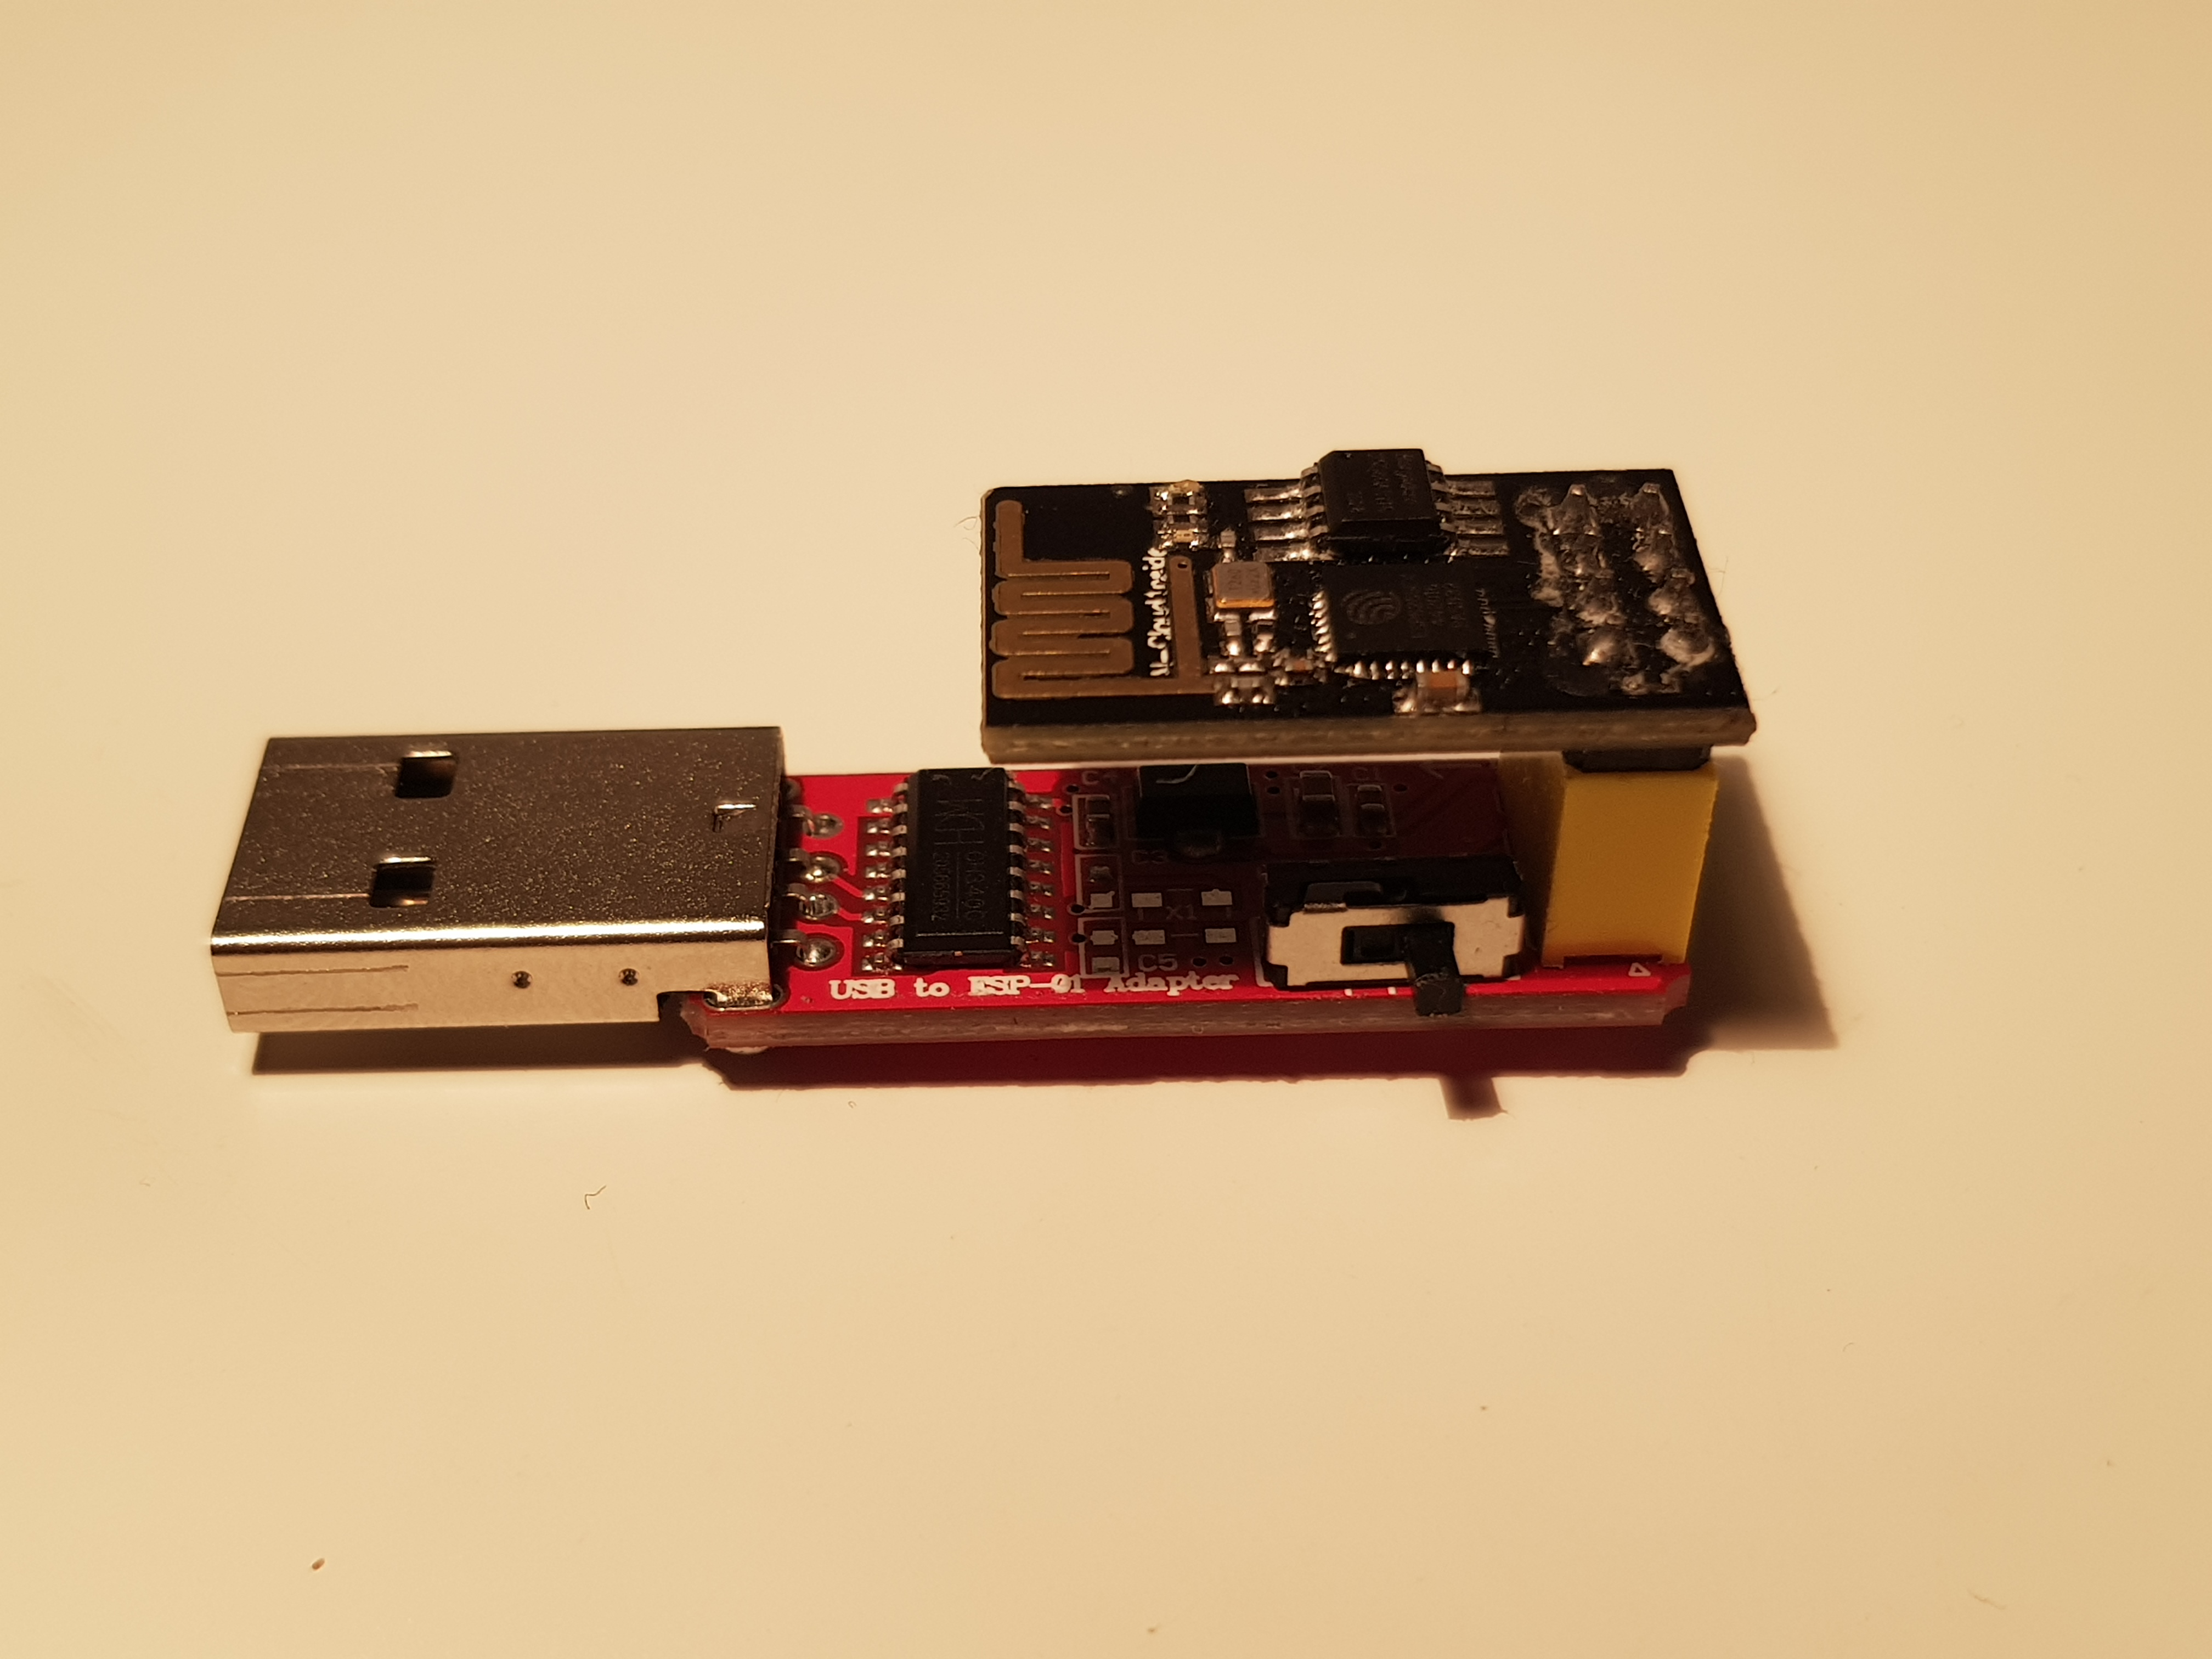
\includegraphics[width=0.5\textwidth]{imagenes/programador.jpg}
\label{fig:programador}
\caption{Adaptador TTL-USB CP2102}
\end{figure}

\begin{figure}
\center
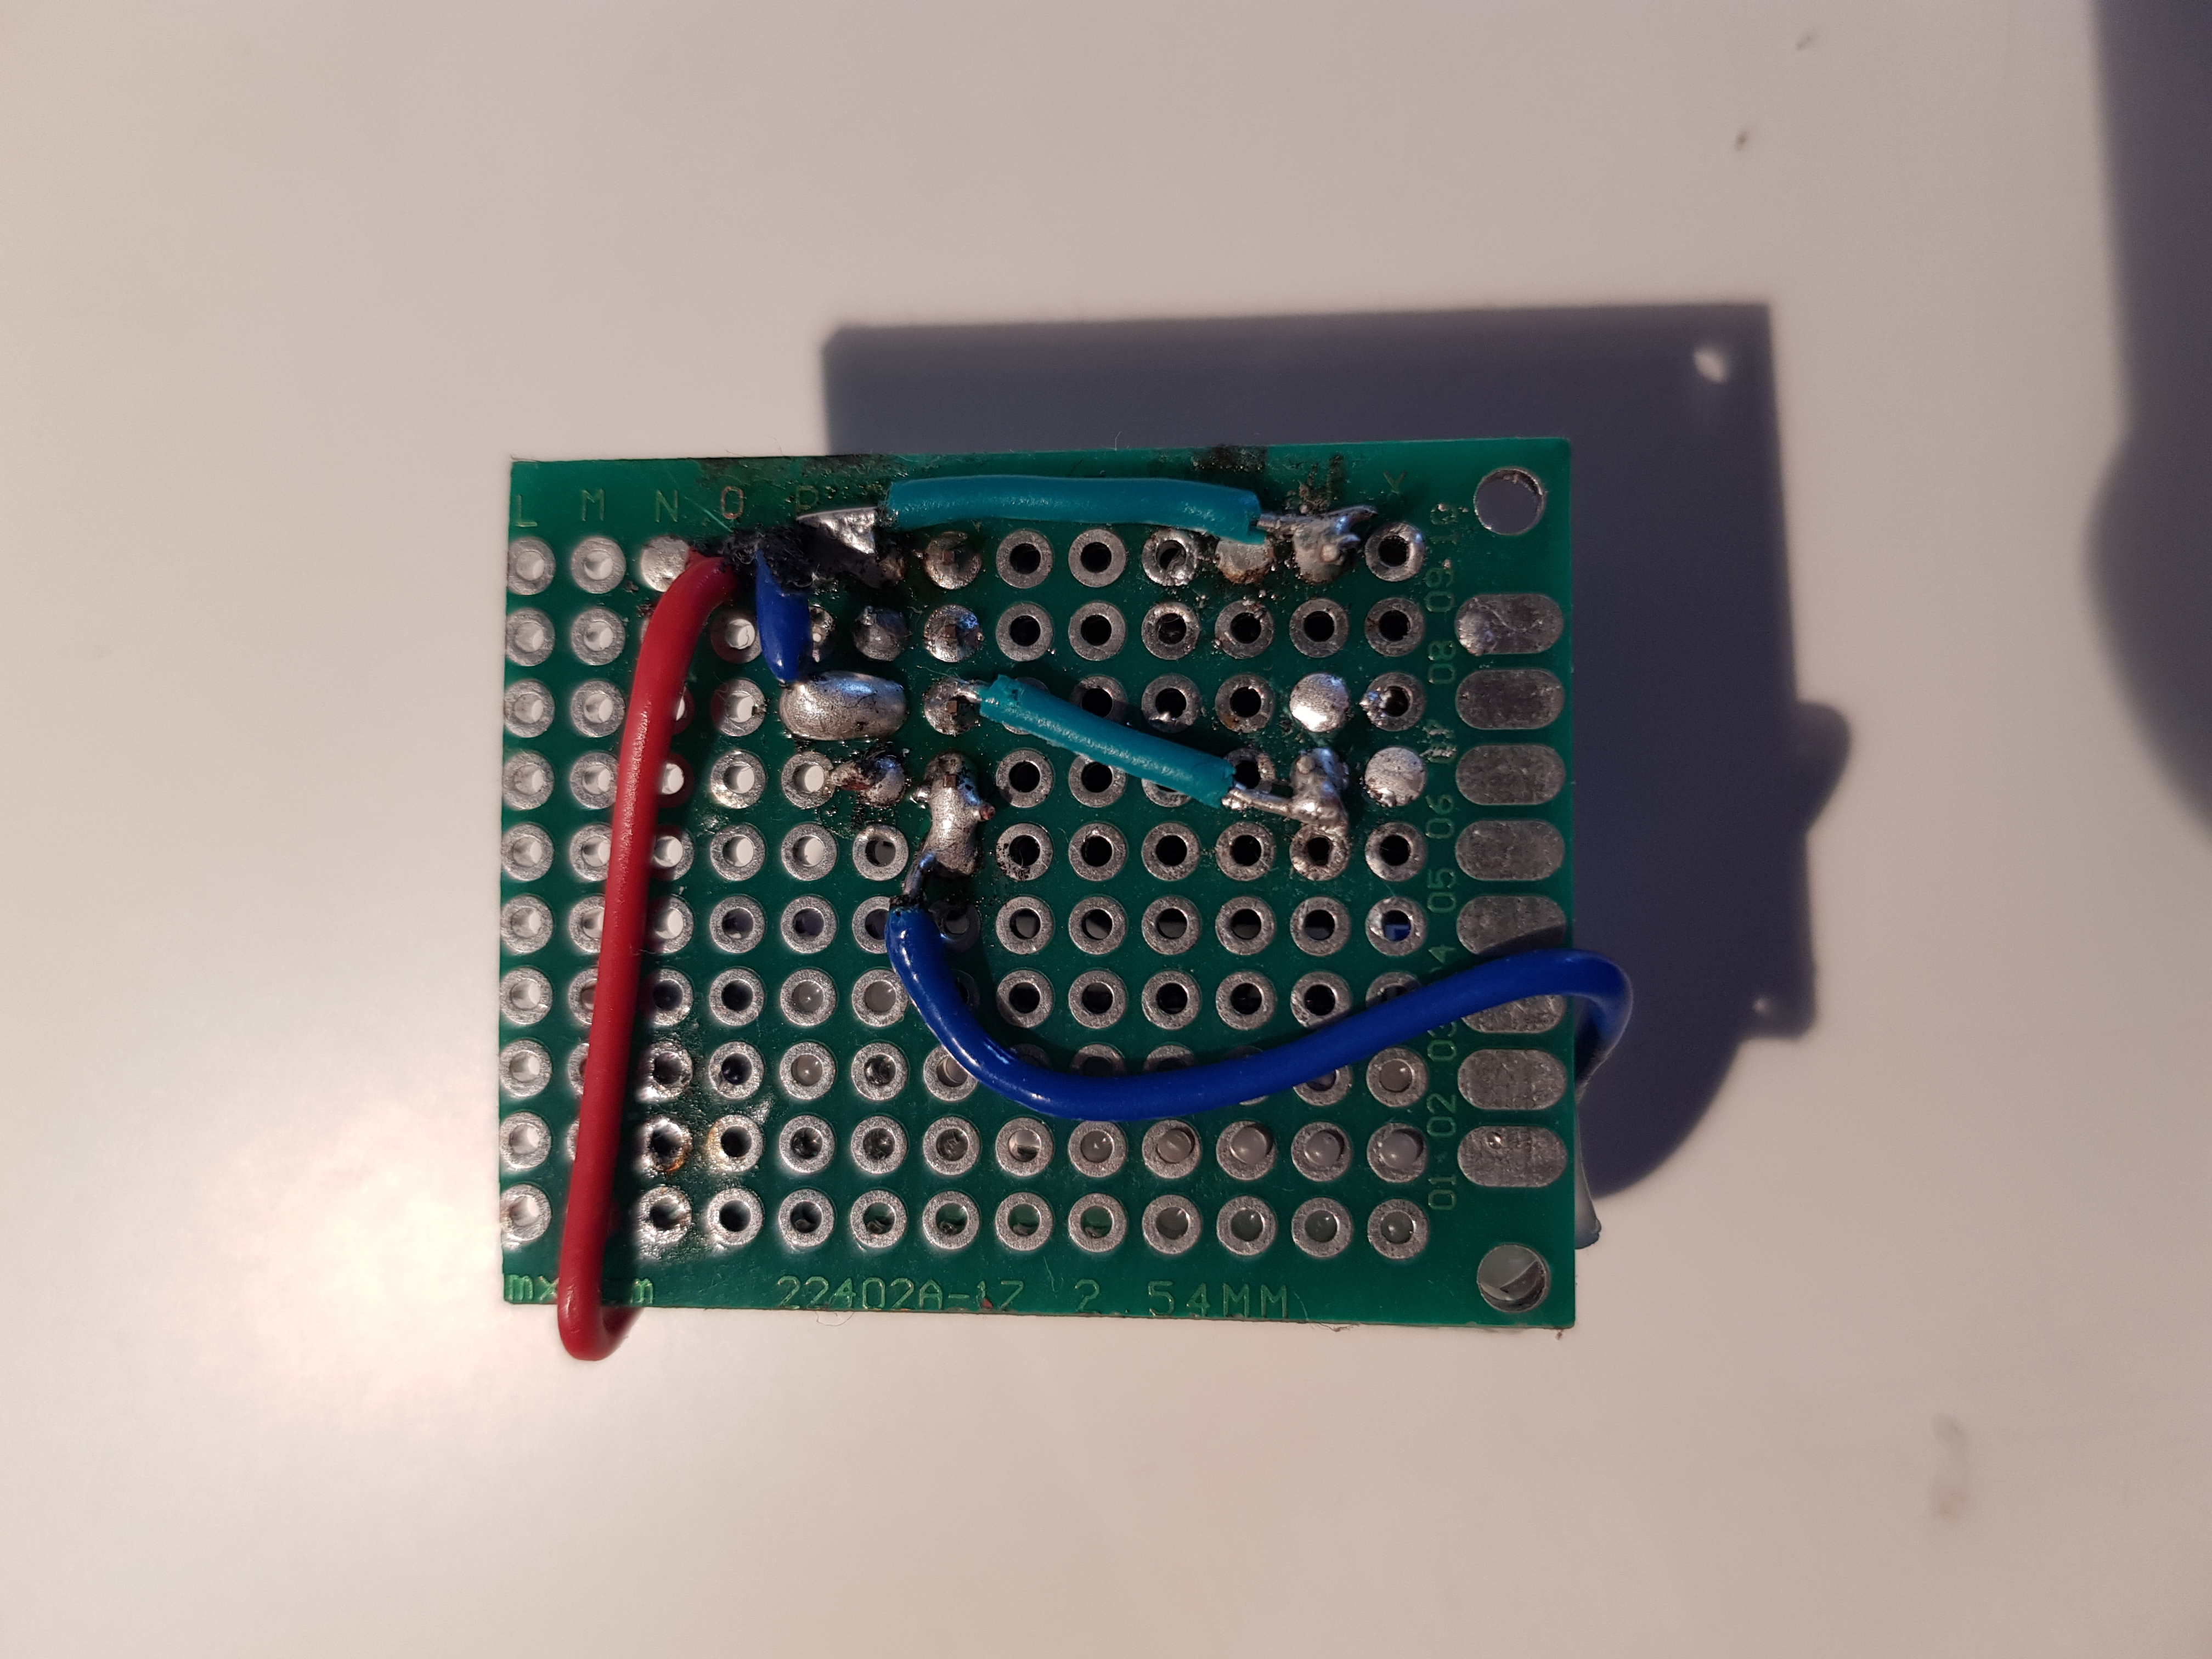
\includegraphics[width=0.5\textwidth]{imagenes/reverso.jpg}
\label{fig:reverso}
\caption{Reverso de la placa}
\end{figure}



\section{Nodo relé}
El funcionamiento de este nodo es muy simple: activa o desactiva un relé dependiendo del mensaje que le llegue por el protocolo MQTT. Para el hardware se ha utilizado producto \textit{Sonoff Basic}, que es dispositivo con carcasa listo para instalarlo en una vivienda. La ventajas de utilizar este frente a crearlo a partir de los componentes son: 
\begin{itemize}
\item Le recubre una carcasa, dándole aspecto de un producto acabado.  
\item Incluye una conversor de red electrica (220V) a una tensión que más adecuada para la electrónica digital (3.3V). 
\item El microcontrolador es un ESP8266, por lo se puede programar de la misma manera que los demás nodos.
\end{itemize}
\begin{figure}
\center
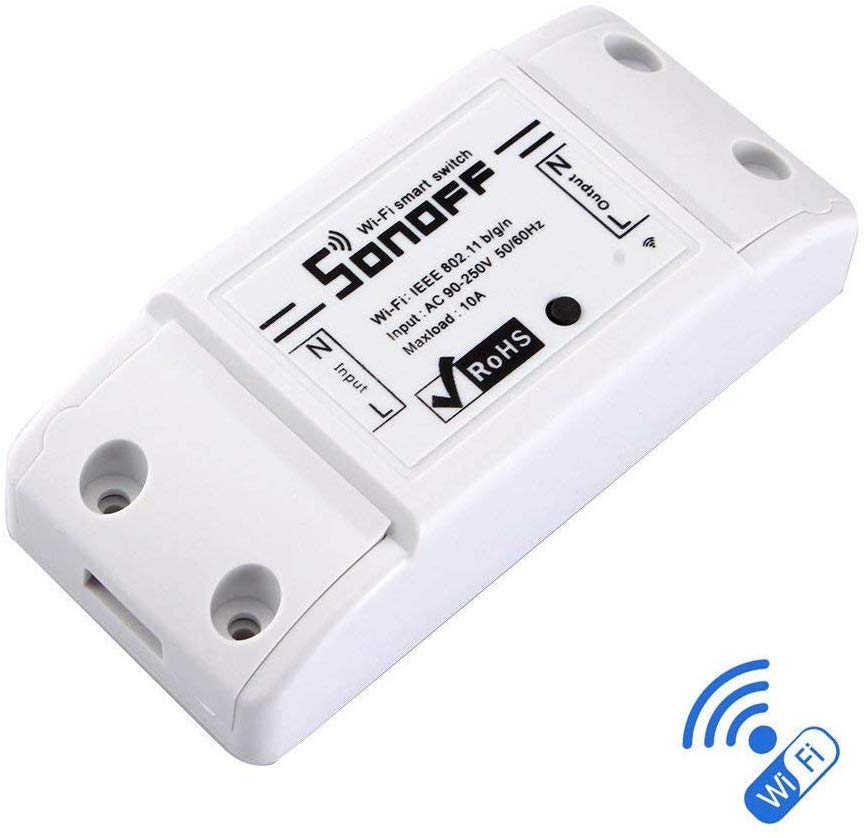
\includegraphics[width=0.5\textwidth]{imagenes/sonoff.jpg}
\label{fig:sonoff}
\caption{\textit{Sonoff Basic}}
\end{figure}
El software de fábrica necesita conectarse mediante una aplicación de smartphone llamada \textit{eWeLink}
. Con ella se puede configurar el horario de activación, pero no resulta util para integrarlo en este proyecto, por lo que se ha tenido que cambiar su firmware. Esto lleva a la necesidad de desmontar el dispositivo y buscar los pines listados en la siguiente tabla:  
\begin{center}
\begin{tabular}{|c|l|}
\hline
Vcc & Alimentación de 3.3V\\
\hline
GND & Tierra\\
\hline
Tx & Transmisión por UART\\
\hline
Rx & 			  Recepción por UART\\
\hline
GPIO0 & \hspace*{-0.2cm}\begin{tabular}{l}Este pin se conecta a tierra \\
			  en el momento que se alimenta\\
			  el microcontrolador para que \\
			  se active el modo programación
			  \end{tabular}\\
\hline
\end{tabular}
\end{center}
Los 4 primeros pines se encuentran juntos y alineados como se muestra en la figura \ref{fig:pines}. El pin GPIO se encuentra conectado a un botón. 
\begin{figure}
\center
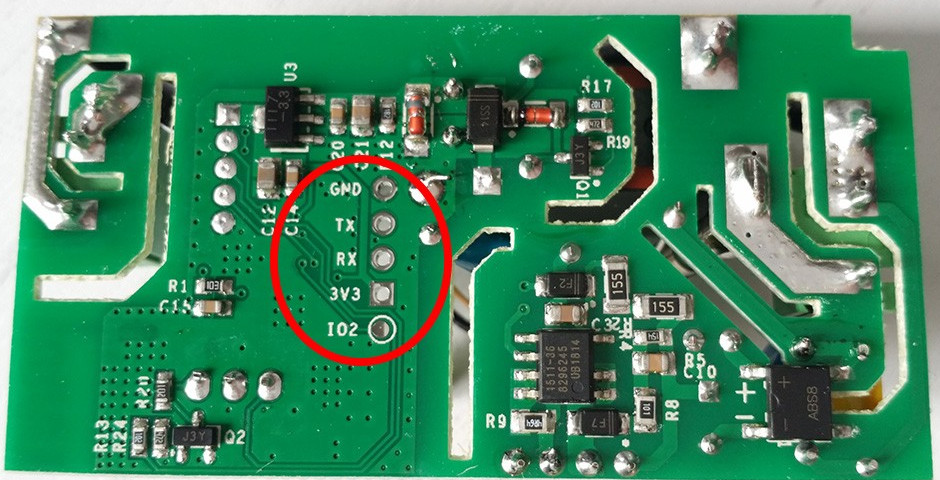
\includegraphics[width=0.5\textwidth]{imagenes/pines.jpg}
\label{fig:pines}
\caption{Pines para reprogramar el ESP8266}
\end{figure}

\end{document}
